\section{Introduction}~\label{sec:introduction}

\todo{Spiel about reversible computing and logical reversibility}
\todo{Spiel about using groupoids for denotational semantics}

\paragraph*{Synthesis of Reversible Core of Quantum Circuits.}

Most current quantum algorithms start with generating superpositions, evolving them using a unitary transformation, and then projecting them with a measurement operator. The middle stage is essentially a reversible classical computation (executed in a quantum-parallel fashion). We illustrate that middle stage in detail by synthesizing a reversible circuit implementing boolean disjunction ($\vee$). Following~\citet{Toffoli:1980}, the first step is to write a specification for the desired reversible function:
\[
\mathit{reversibleOr}(h,b_1,b_2) ~=~ (h \,\underline{\vee}\, (b_1 \vee b_2), ~b_1, ~b_2)
\]
where $\underline{\vee}$ is the exclusive-or operation. From the definition of $\underline{\vee}$ it is evident that setting $h=0$, we can compute the desired disjunction by observing the first component of the result. The $\mathit{reversibleOr}$ function has the following truth table (in binary on the left and in a more convenient decimal notation on the right):

\begin{center}\begin{tabular}{|ccc|ccc|@{\qquad\qquad}|c|c|}
0 & 0 & 0 &     0 & 0 & 0     & 0 & 0 \\
0 & 0 & 1 &     1 & 0 & 1     & 1 & 5 \\
0 & 1 & 0 &     1 & 1 & 0    & 2 & 6 \\
0 & 1 & 1 &     1 & 1 & 1    & 3 & 7 \\
1 & 0 & 0 &     1 & 0 & 0    & 4 & 4 \\
1 & 0 & 1 &     0 & 0 & 1    & 5 & 1 \\
1 & 1 & 0 &     0 & 1 & 0    & 6 & 2 \\
1 & 1 & 1 &     0 & 1 & 1    & 7 & 3
\end{tabular}\end{center}

\noindent where it is evident that it is a bijective function, i.e., reversible.

The above embedding of an irreversible function into a reversible function with additional inputs and outputs is completely general and is the starting point for specifications of quantum circuits. The challenge is to synthesize a program / circuit from this specification. Of course, writing this program in a conventional (irreversible) language defeats the purpose. The challenge is to construct the desired program / circuit exclusively using reversible primitives, e.g., the standard set of universal reversible gates used in frameworks like Qiskit which consists of the computational gates \textsf{not} (boolean negation, called \verb|x|), \textsf{cnot} (conditional negation of the second input if the first is true; called \verb|cx|), and \textsf{toffoli} (conditional negation of the third input if both the first two inputs are true; called \verb|ccx|) gates, and the ability re-arrange the layout of wires. For concretness, here is a possible implementation of the desired function in Qiskit:

\begin{center}
  \begin{minipage}[c]{0.4\linewidth}
\begin{verbatim}
reversibleOr.qasm:

  // setup
  ccx q[1], q[2], q[0];
  cx  q[1], q[0];
  cx  q[2], q[0];
  // measure

% ./qasm -t reversibleOr.qasm
+-------+-------+
| 0 0 0 | 0 0 0 |
| 0 0 1 | 1 0 1 |
| 0 1 0 | 1 1 0 |
| 0 1 1 | 1 1 1 |
| 1 0 0 | 1 0 0 |
| 1 0 1 | 0 0 1 |
| 1 1 0 | 0 1 0 |
| 1 1 1 | 0 1 1 |
+-------+-------+
  \end{verbatim}
  \end{minipage}
  \qquad
  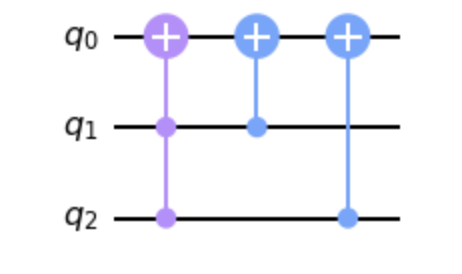
\includegraphics[scale=0.7]{reversibleOr.png}
\end{center}

This implementation was manually produced using a standard synthesis algorithm for reversible circuits~\cite{10.1145/775832.775915}. To gain some intuition, we trace the evaluation of the circuit for input \verb|011|. In this context, the most significant bit is at index 0. Thus the first \verb|ccx| gate negates \verb|q[0]| since both \verb|q[1]| and \verb|q[2]| are true producing \verb|111|; the following \verb|cx| gate negates produces \verb|011|; finally the last \verb|cx| produces the final result \verb|111|.

There is wealth of manual and algorithmic approaches for such synthesis problems each optimizing along  different dimensions~\cite{XXX}. Here is the circuiit produced using an approach that analyzes the recursive structure of the circuit (and would generalize to computing the disjunction of more than two inputs):

\begin{center}
  \begin{minipage}[c]{0.4\linewidth}
\begin{verbatim}
reversibleOr2.qasm:

  // setup
  cx  q[1], q[0];
  x   q[1];
  ccx q[1], q[2], q[0];
  x   q[1];
  // measure
  \end{verbatim}
  \end{minipage}
  \qquad
  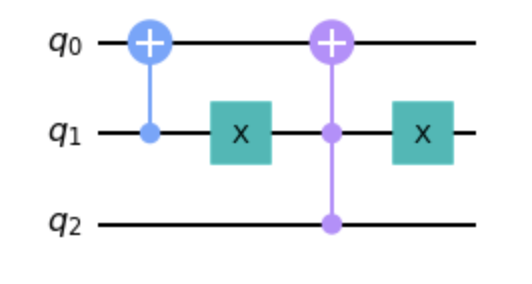
\includegraphics[scale=0.7]{reversibleOr2.png}
\end{center}

The evaluation of this circuit prints the same truth table as above confirming their equivalence. Tracing the evaluation on the same value \verb|111| goes through the stages \verb|011|, \verb|111|, \verb|101|, \verb|101|, and finally \verb|111|.

The situation for Shor's algorithm is just as described above but with a more involved function of the form $f(r) = a^{r} \mod N$ for fixed $a$ and $N$. The specification of the circuit is relatively straightforward to calculate. Here it is for $a=11$ and $N=15$:
\[\begin{array}{rcll}
g(r,h) &=& (r,h+1) & \mbox{when~$r$~even~and~$h$~even} \\
(r,h) &=& (r,h-1) & \mbox{when~$r$~even~and~$h$~odd} \\
g(r,h) &=& (r,11-h) & \mbox{when~$r$~odd~and~$4 > h \geq 0$~or~$12 > h \geq 8$} \\
g(r,h) &=& (r,19-h) & \mbox{when~$r$~odd~and~$8 > h \geq 4$~or~$16 > h \geq 12$}
\end{array}\]
However, as explained in standard accounts of the algorithm (e.g., the Qiskit implementation), such efficient modular exponentiation circuits are not straightforward to derive and are the bottleneck in Shor’s algorithm. Typical derivations of the circuit start from elementary gates, build a circuit for modular addition, which is used to build a circuit for modular multiplication, and then finally a circuit for modular exponentiation taking care at each step to avoid the exponential blowup~\cite{shorefficient}.

\paragraph*{Our Technical Results.}



synthesis algorithms (no correctness)

programming from sccratch (manual / perhaps better; also no correctness embedded)

for complex circuits correctness not evident


The circuit must be built from reversible primitives and guaranteed to have the same functionality as the original bijective function.

It would be good if we could write a 3 way correspondence in a table like this, but I'm not sure where:

Pi types -- Natural number -- Finite sets
1-combinator -- Generators of Sn -- 1-paths
2-combinator -- Relations of Sn -- 2-paths

This review does make me very nervous, basically all we've done is taken MacLane's coherence theorem and formalised it in HoTT, and given presentations for it using Pi's syntax. There's nothing "new", but the new idea is that we can use this for reversible circuit equivalence and normalisation.

But we do have a complete proof that UFin is the free sym. mon. groupoid, which wasn't there earlier

Wouldn't it be simpler to write this permutation and automatically derive a circuit from it? This is exactly what we accomplish. We can take the permutation above, generate a circuit from it, \emph{and most importantly} generate a proof of correctness along with the circuit. As part of the infrastructure we provide a sound and complete calculus of reversible functions that can be used to (i) generate circuits from permutations like above, (ii) translate circuits to a normal form, (iii) reason about equivalence of circuits, (iv) and provide a framework for reasoning about trade-offs among optimizing tranformations.

Technically, the main result is a soundness and completeness theorem relating a 2-level reversible programming language with a univalent universe of finite types expressed as a weak groupoid in the metalanguage of HoTT. On the HoTT we start with a univalent subuniverse specification of finite types, equivalences between them, and homotopies between the equivalences. This is a concise description of everything we need to know about circuits and transformations among them. Along the way, we \ldots \note{copy relevant pieces from below}


\note{Could we include a short paragraph about entropy and bits and logical reversibility?}

 Referee 4 states that "The main result of the paper is that the
  category of finite sets and bijections, with the two monoidal
  structures given by sum and product, is the free rig groupoid."

  Indeed some of the connections above are trivial in "conventional
mathematics"; however some of those same connections hide implicit
isomorphisms (changes of representations) that are important
computationally.  Our construction shows, for example, that
transporting properties across equivalences of finite types can be
done via executing permutations, something which has a clear
computational cost and which itself depends on the choice of
representations of the permutations.

\subsection*{A Complete Example}




\subsection*{Outline and Contributions}

\begin{itemize}[leftmargin=*]
\item We take the $\PiLang$ family of reversible languages~\cite{jamesInformationEffects2012} and show how to encode various boolean reversible circuits in the language. The circuits are implemented using 1-combinators in the language, and circuit optimisations are realised as 2-combinators between these reversible programs.
\item We show how to encode reversible circuits on a fixed number of bits as permutations of finite sets with the appropriate cardinality. We observe that reversible programs can be translated to bijective functions between finite sets and equality of reversible programs can be witnessed as extensional equality of these bijective functions, which is decidable.
\item We review a few basics of Homotopy Type Theory~\cite{univalentfoundationsprogramHomotopyTypeTheory2013}, and exhibit some results that we use in our technical development. We define the notion of a universe \`{a} la Tarski internally in HoTT, which is given by a type for codes $U$ and a decoding function to a univalent universe $\El : U \to \UU$. We say that this universe is univalent, if the decoding fibration is univalent, that is, the decoding function $\El$ reflects the path space of the underlying univalent universe. We exhibit some examples of univalent subuniverses, in particular, we define the subuniverse of finite types, $\UFin$, which classifies all types with a specified cardinality $n : \Nat$, and show that it is univalent. Hence, we establish a characterisation of the path space of the universe of finite types.
\item We observe that 1-paths in $\UFin$ are permutations on finite sets with a fixed cardinality $n$, given by $\Aut[\Fin[n]]$. We define Lehmer codes~\cite{lehmerTeachingCombinatorialTricks1960} for permutations, which are a convenient and compact representation of permutations. We show that there is an equivalence between Lehmer codes and permutations $\Lehmer[n] \eqv \Aut[\Fin[n]]$ given by the Lehmer encode-decode algorithm.
\item Then, we give a presentation of the symmetric group $\Sn[n]$ on $n$ generators, given by the set-quotient of $\List[\Fin[n]]$ by Coxeter relations. We define the short form and long form of the Coxeter relations for the symmetric group, and show that the long form of the relation is (locally) confluent and strongly normalising, and that both the forms are equivalent. From this, we show that the Coxeter relation produces a normal form for words in $\Sn$. We further show that this indeed gives a group presentation for $\Sn$, and that we can decode a Lehmer code to a word in $\Sn[n]$ and back, giving the equivalence $\Sn[n] \eqv \Lehmer[n]$. This gives an axiomatisation of permutations on $\Fin[n]$ as relations on $\List[Fin[n]]$, which we use to interpret our language $\PiLang$ in our model.
\item Then, we show that $\UFin$ has a symmetric monoidal structure (the additive one), where the unit is given by the empty set, and the tensor product of two finite sets is given by their disjoint union. We show that this satisfies the associator, unitor and symmetry isomorphisms of a symmetric monoidal category, and Mac Lane's pentagon, hexagon, and syllepsis coherence conditions. This gives a complete characterisation of our model $\UFin$ which we interpret our language $\PiLang$ into.
\item Finally, we interpret the language $\PiLang$ into our model. First we define a subset of the language $\PiPlusLang$ which only includes the additive monoidal structure. Then, we define a normalised form for this language in $\PiHatLang$, where the objects of the language are simply the unary natural numbers, and give normalised 1-combinators and 2-combinators which perform adjacent transpositions.
\item We show how to interpret this language $\PiHatLang$ into $\UFin$, translating the natural numbers into the cardinality of the finite set, 1-combinators into permutations via words in $\Sn$, and 2-combinators as 2-paths in $\UFin$. We further show how to quote back a permutation in $\UFin$ into a 1-combinator using the normal form for words in $\Sn$. We show that this gives a symmetric monoidal equivalence.
\item Then, we show that $\PiPlusLang$ can be translated into $\PiHatLang$. The 1-combinators are translated as composition of adjacent transpositions, and the 2-combinators are interpreted using the coherence conditions for symmetric monoidal categories. We further show that this translation can be inverted, giving a symmetric monoidal equivalence.
\item Finally, we give a translation from $\PiLang$ to $\PiHatLang$ and $\PiLang$, using the additive structure and distributivity to build the multiplicative structure. We show that this translation reflects 2-combinators. We give some applications of this translation by showing how to normalise a circuit written in $\PiLang$ to a normal form in $\PiPlusLang$ and $\PiHatLang$, which uses fewer gates.
\end{itemize}

Our results are formalised in the proof assistant Agda using the HoTT-Agda library.

\note{Novel interpretation of the univalence axiom, operational and denotational semantics and adequacy.}

\begin{center}
  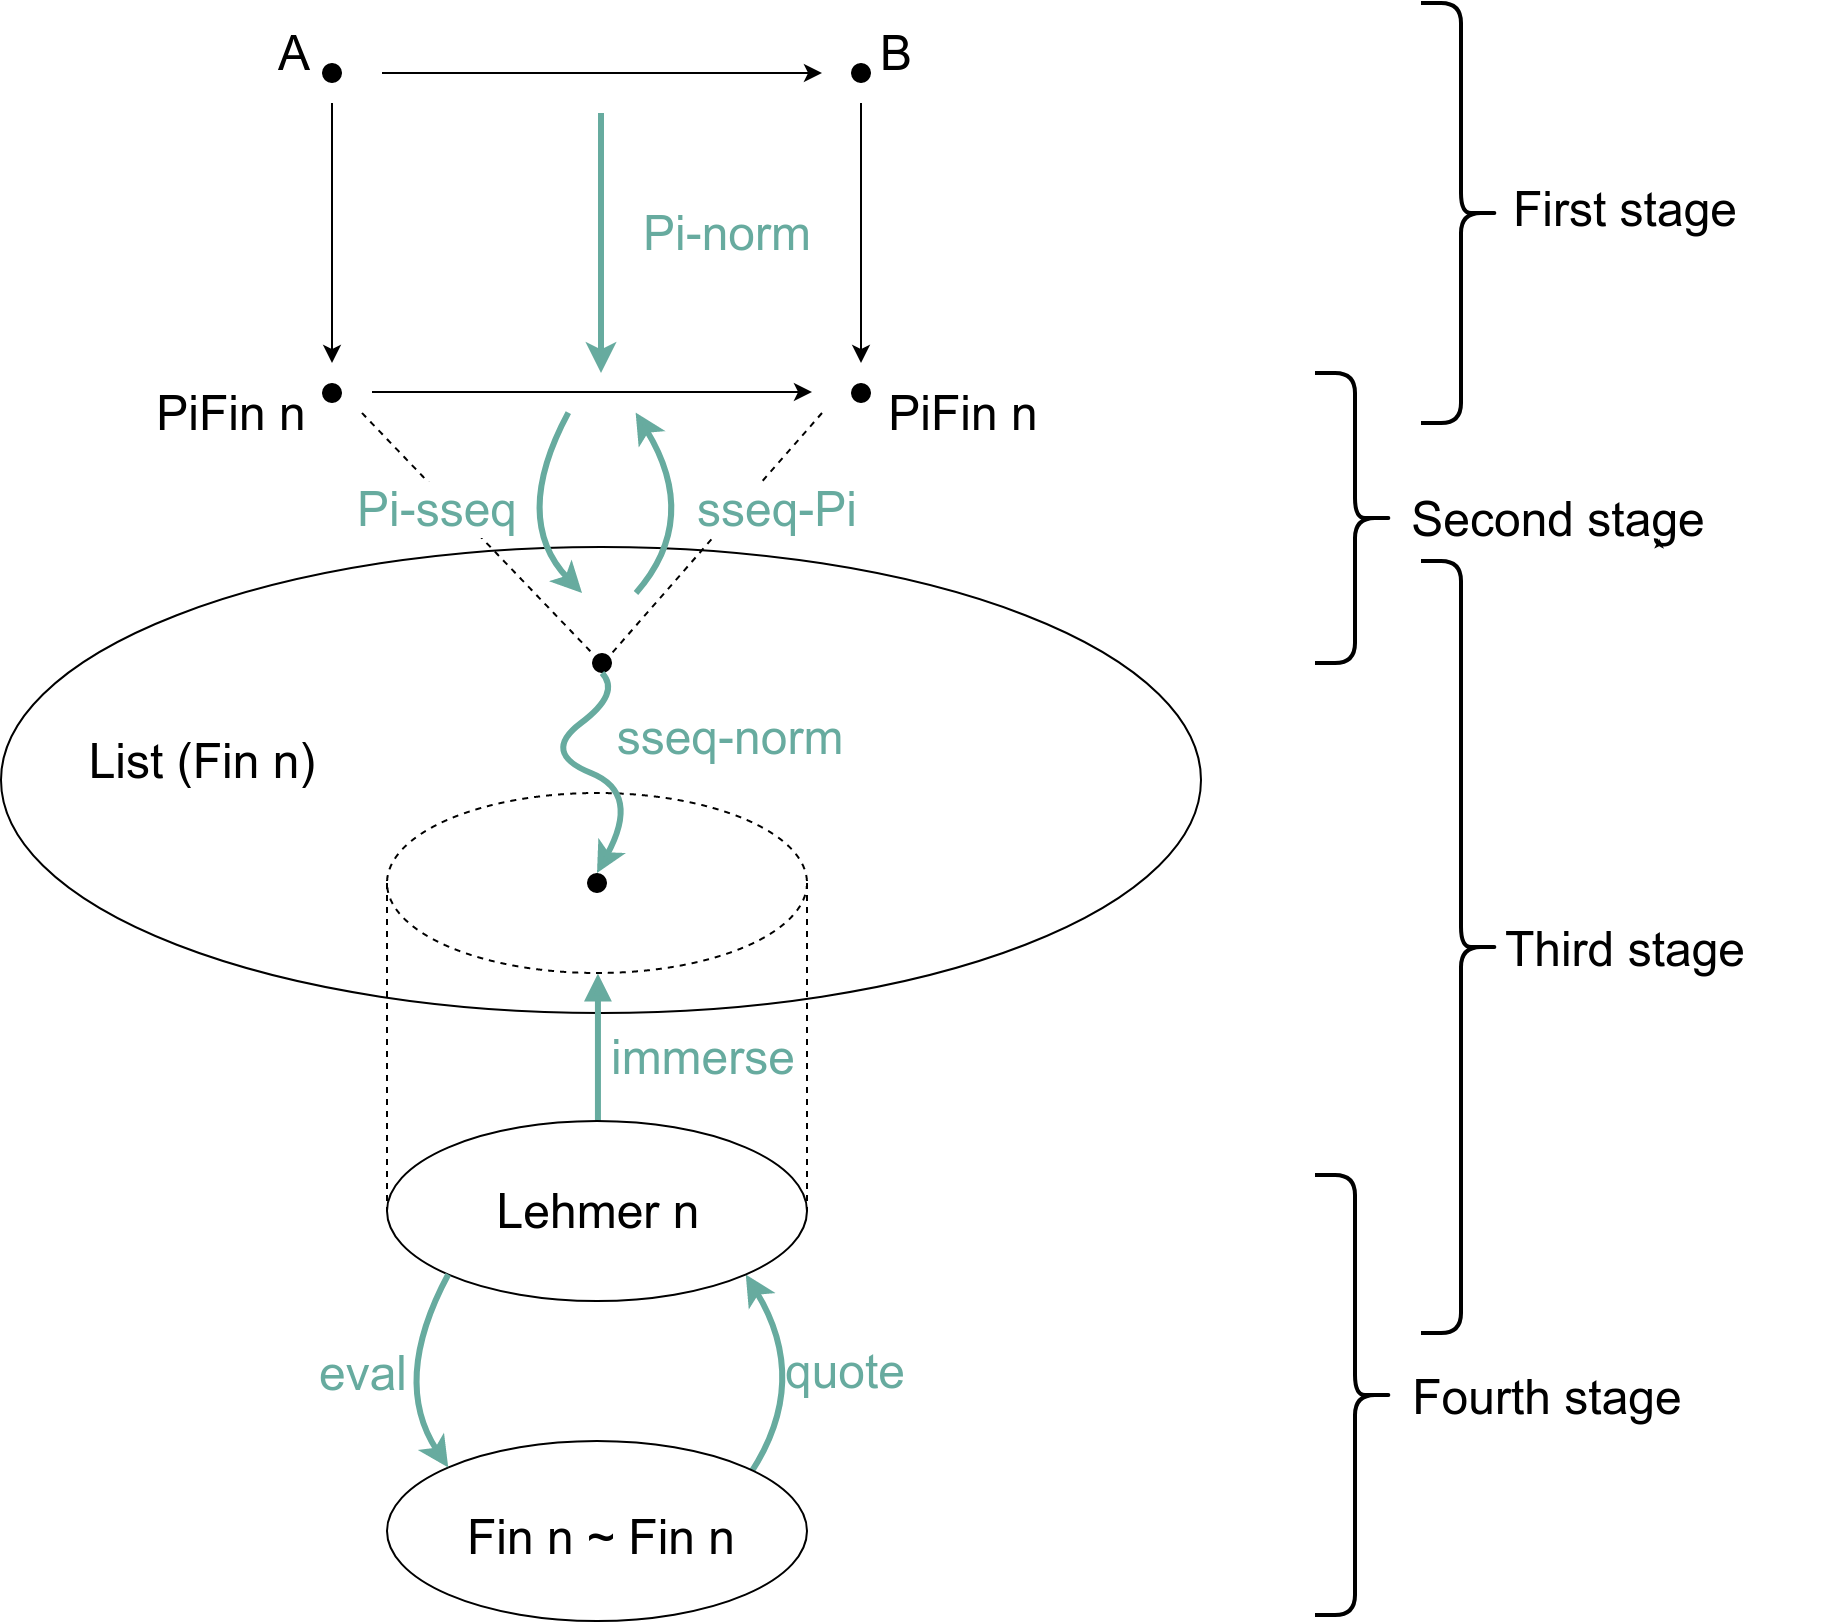
\includegraphics[scale=0.3]{outline.png}
\end{center}


%%% Local Variables:
%%% mode: latex
%%% TeX-master: "main"
%%% fill-column: 120
%%% End:
